\section{Resultados}
\label{resultados}

En esta sección se va a mostrar los resultados obtenidos con este proyecto, además de explicar como afecta cada uno de los distintos parámetros del algoritmo al tiempo de computo total y a la obtención del camino.\\

Lo primero que hay que decir es que el conjunto del programa funciona como es debido, es decir, si los parámetros del algoritmo tienen los valores adecuados, genera el grafo con las conexiones adecuadas, encuentra el camino más corto, en caso de que exista uno, y envía todos los datos al simulador, que se encargará de mover al robot al punto indicado. Esto se ha comprobado para los tres escenarios descritos en el apartado 4.1, usando varias configuraciones distintas y los dos algoritmos de búsqueda implementados. Respecto a esto último, cabe decir que, mientras que el Dijkstra siempre encuentra un camino si es posible, el $A^*$ puede no encontrarlo. Esto en teoría no debería ocurrir, ya que ambos algoritmos son completos, es decir, siempre deberían devolver una solución en caso de que exista, por lo que lo mas probable es que se deba a un problema en la implementación del $A*$.\\

En cuanto al estudio que tienen los diferentes parámetros sobre el resultado final, se va a realizar un analisis sobre cinco factores: el número de nodos, el valor elegido como umbral para la búsqueda de vecinos, el tipo de conjunto de datos empleado, el algoritmo de búsqueda utilizado y el comprobador de colisiones elegido. Para cada caso, el resto de parámetros se mantendrán con el mismo valor que en el caso de control, que en este caso tiene los siguientes valores:\\

\begin{enumerate}
\item Número de nodos: 500.
\item Valor elegido como umbral: 50
\item Comprobador de colisiones elegido: dilate
\item Tipo de puntos: Hammersley
\item Algoritmo de búsqueda: $A^*$
\item Escenario elegido: Escenario B
\end{enumerate}

\subsection{Efecto del número de nodos}

Para este primer experimento, se variará el número de puntos que se usan para muestrear el espacio libre, manteniendo los otros parámetros, y se calculará el tiempo que tarda el programa en ejecutarse desde que se lanza hasta que se encuentra el camino (no se tiene en cuenta el tiempo que tarda el robot en moverse). Esto se probará para los siguientes valores: 50, 100, 500, 1000, 5000.\\

Teóricamente, un menor número de nodos implica que habrá grandes regiones del espacio de soluciones que no se estén comprobando, lo que llevará a que no existan conexiones entre nodos, por lo que probablemente no sea posible encontrar un camino entre los puntos inicial y final.  En la figura \ref{fig:nodos_vs_t} se puede observar los resultados obtenidos.

\begin{figure}[H]
		\centering
        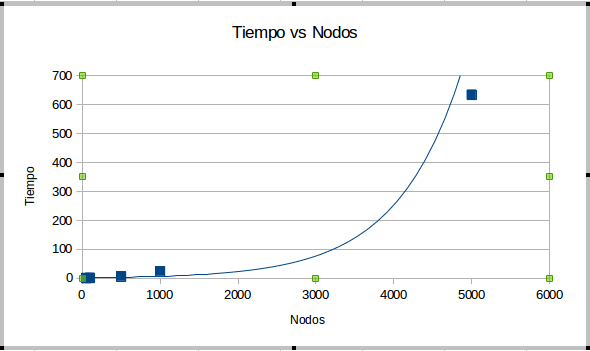
\includegraphics[width=0.2\textwidth]{images/t_vs_nodos.png}
        \caption{Número de nodos frente al tiempo}
        \label{fig:nodos_vs_t}
\end{figure} 

Se puede ver como el tiempo de calculo crece de forma exponencial al aumentar el número de nodos. Esto se debe a que, a mayor número de nodos, más colisiones hay que comprobar, y aumenta el número de vecinos de cada nodo, lo que implica más trabajo para el algoritmo de búsqueda. Además, con esta configuración, el programa fué incapaz de encontrar un camino para 50 y para 100 nodos, mientras que en los otros tres casos si que existió una trayectoria. Es más, con 50 nodos, ni siquiera fué posible establecer conexiones entre estos, ya que se encontraban demasiado alejados. En la figura \ref{fig:nodos_vs_t} se puede observar como varía el muestreo en funcion del número de nodos. Estos resultados prueban lo que ya se esperaba obtener, además de dar una idea de la importancia que tiene este parámetro.\\ 

\begin{figure}[h]
		\centering
        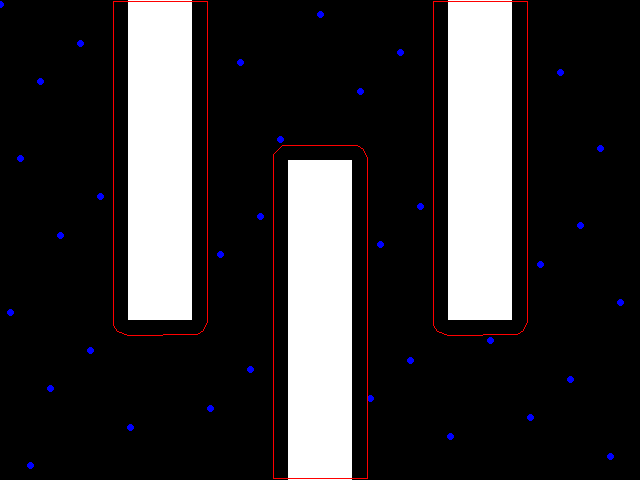
\includegraphics[width=0.35\textwidth]{images/50puntos.png}
        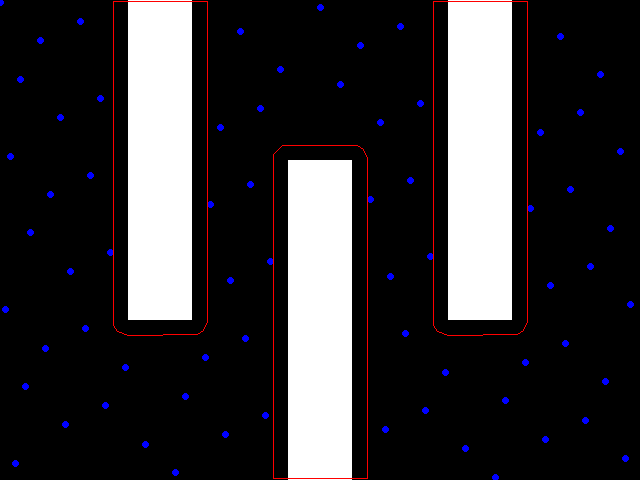
\includegraphics[width=0.35\textwidth]{images/100puntos.png}
        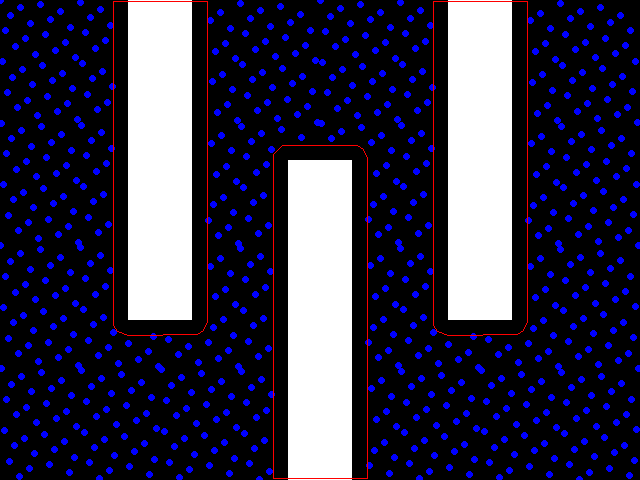
\includegraphics[width=0.35\textwidth]{images/1000puntos.png}
        \caption{Variación en el muestreo en funcion del número de puntos (50, 100, 1000)}
        \label{fig:50_100_1000nodos}
\end{figure}  

\subsection{Efecto del valor del umbral}

El umbral es el parámetro que controla cual es la distancia máxima a la que dos nodos vecinos pueden estar. Si se elige un valor muy bajo, a menos que se trabaje con un gran número de nodos, no existirán suficientes conexiones como para asegurar la existencia de un camino, mientras que si el ubral es muy alto, todos los nodos estarán conectados entre si y será mucho mas pesado computacionalmente calcular el camino más corto. Al igual que antes, se mantendrán todos los parámetros con el valor del caso de control, y se irá variando el valor del umbral, en este caso 50, 100, 200, 300, 400 y 500. En la figura \ref{fig:umbral_vs_t} se pueden observar los resultados:\\

\begin{figure}[H]
		\centering
        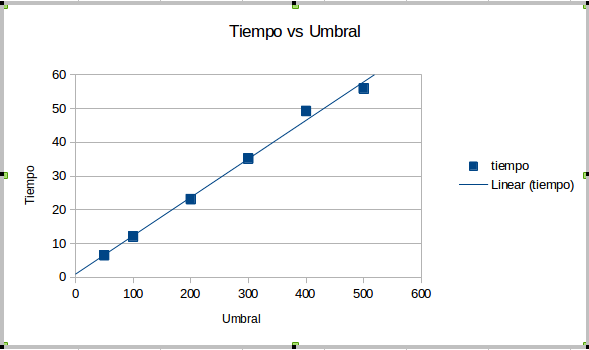
\includegraphics[width=0.2\textwidth]{images/t_vs_umbral.png}
        \caption{Valor del umbral frente al tiempo}
        \label{fig:umbral_vs_t}
\end{figure}

Se puede observar como el coste computacional crece de forma lineal con el valor del umbral, aunque al llegar a un determinado valor dejará de crecer y se mantendrá estable, dado que el umbral será tan amplio que todos los nodos serán vecinos unos de otros. De este apartado y del anterior se extrae la conclusión de que el número de nodos y el valor del umbral son dos parámetros que están estrechamente relacionados, por lo que es necesario ajustarlos con precisión. Si tienes un umbral muy bajo, probablemente sea necesario un gran número de nodos para encontrar el camino, y viceversa. Dados los resultados que se han visto, es preferible trabajar con menos nodos y un umbral más alto, de cara a reducir el tiempo de cálculo. En la figura \ref{fig:50_100_300umbral}

\begin{figure}[h]
		\centering
        \includegraphics[width=0.35\textwidth]{images/50-500puntos.png}
        \includegraphics[width=0.35\textwidth]{images/100-500puntos.png}
        \includegraphics[width=0.35\textwidth]{images/300-500puntos.png}
        \caption{Variación en la conectividad en funcion del umbral (50, 100, 300)}
        \label{fig:50_100_300umbral}
\end{figure}

\subsection{Efecto del algoritmo de busqueda}

Para este proyecto se han implementado dos algoritmos para encontrar el camino óptimo dentro del grafo, el $A^*$ y el Dijkstra, para poder analizar como esto afecta al resultado total. A priori, este es uno de los cuellos de botella del proceso, junto con la comprobación de colisiones. Dado que no es necesario un algoritmo en concreto, lo mejor sería buscar entre todas las posibles opciones aquella que encuentre el mejor camino en el menor tiempo posible.\\

Se variará el número de nodos y se medirá el tiempo que tarda cada algoritmo encontrar una solución (si existe). En la figura \ref{t_vs_alg} se pueden ver los resultados obtenidos:\\

\begin{figure}[H]
		\centering
        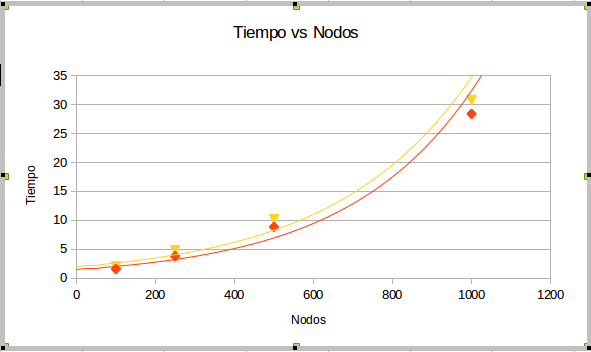
\includegraphics[width=0.2\textwidth]{images/t_vs_nodos_vs_alg.png}
        \caption{Tiempo necesario para hallar un camino}
        \label{fig:t_vs_alg}
\end{figure}

Donde las muestras rojas corresponden al algoritmo $A^*$ y las amarillas, al Dijkstra. Por lo general, no existe una diferencia substancial en el tiempo de ejecución, puede estar alrededor de 1-2 segundos, pero esto entra dentro del margen de error de la medida, por lo que la diferencia es despreciable. Sin embargo, como se comentó anteriormente, el Dijkstra encuentra siempre una solución, cosa que no pasa con la implementación que aquí se ha realizado del $A^*$, aunque esto no es propio del algoritmo, por lo que no debería ser un morivo para elegir uno u otro. Por último, con respecto al camino en si, depende del escenario y de los puntos inicial y final elegidos, pero por lo general, el $A^*$ devuelve un camino igual de corto que el Dijkstra, o incluso menor, aunque con la simplificación que se aplica al final del proceso los resultados suelen acabar siendo identicos. Después de estudiar todos estos datos, se puede concluir que el  $A^*$ sería la elección lógica, aunquesin presentar excesivas ventajas. En la figura \ref{comp_paths} se pueden ver las trayectorias que devuelve el  $A^*$, el Dijkstra y la trayectoria simplificada.\\

\begin{figure}[h]
		\centering
        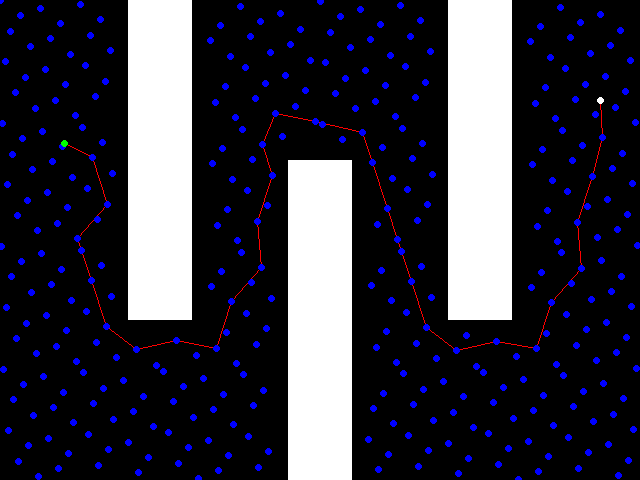
\includegraphics[width=0.35\textwidth]{images/a500.png}
        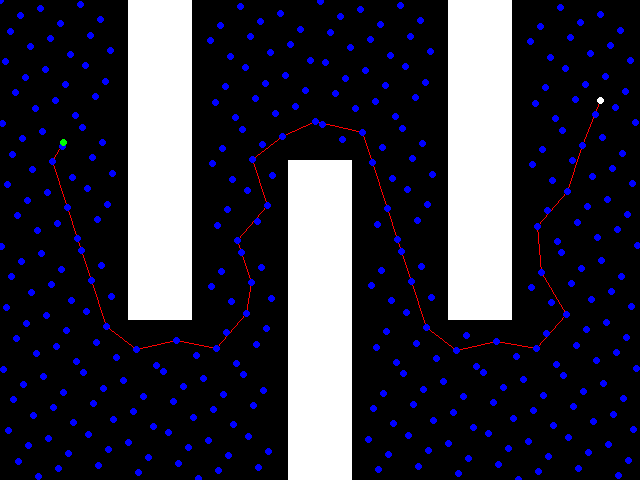
\includegraphics[width=0.35\textwidth]{images/d500.png}
        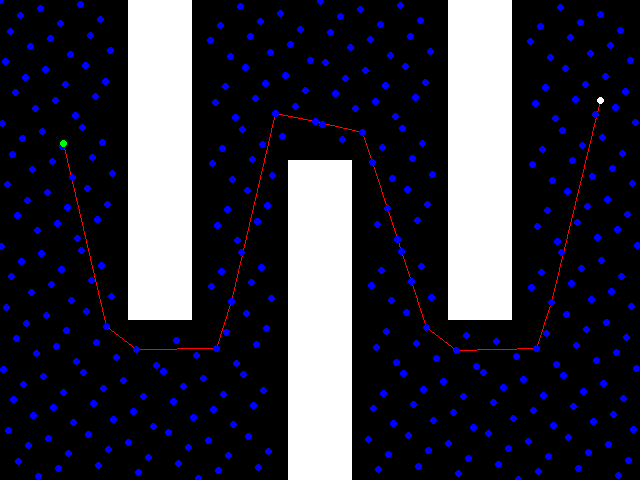
\includegraphics[width=0.35\textwidth]{images/s500.png}
        \caption{Diferentes trayectorias generadas}
        \label{fig:comp_paths}
\end{figure}

\subsection{Efecto del tipo de puntos}

En este proyecto se han usado dos tipos de secuencias de puntos cuasialeatorios (Hammersley y Halton) y un grupo de puntos totalmente aleatorios para poder comparar que efecto tienen. El uso de puntos pseudoaleatorios mejora la exploración del espacio de soluciones, mejorando las posibilidades de encontrar un comino, especialmente en entornos dificiles, con muchos obstáculos o regiones estrechas. En la seccion de implementacion del algoritmo se muestra como muestrea el espacio cada uno de los conjuntos de puntos, Dejando bastante claro que los pseudoaleatorios son      